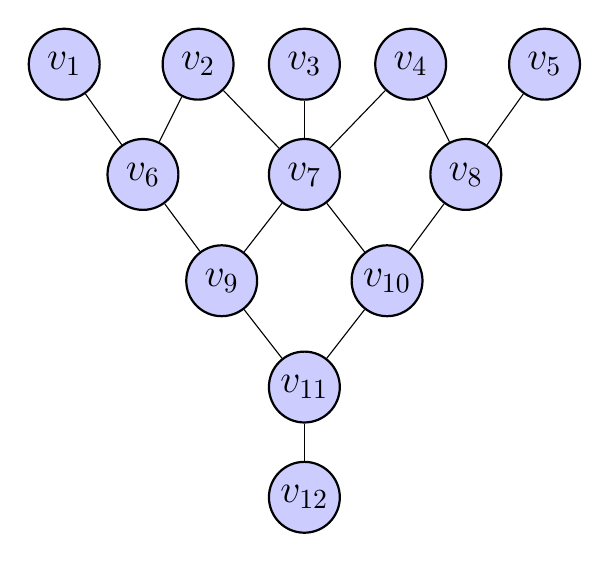
\begin{tikzpicture}[
  scale=1,
  vnode/.style={circle, fill=blue!20, draw=black, thick, minimum size=9mm, inner sep=0pt, font=\Large}
]
  % Vértices
  \node[vnode] (v1)  at (0.4, 5.5) {$v_1$};
  \node[vnode] (v2)  at (2.1, 5.5) {$v_2$};
  \node[vnode] (v3)  at (3.45, 5.5) {$v_3$};
  \node[vnode] (v4)  at (4.8, 5.5) {$v_4$};
  \node[vnode] (v5)  at (6.5, 5.5) {$v_5$};
  \node[vnode] (v6)  at (1.4, 4.1) {$v_6$};
  \node[vnode] (v7)  at (3.45, 4.1) {$v_7$};
  \node[vnode] (v8)  at (5.5, 4.1) {$v_8$};
  \node[vnode] (v9)  at (2.4, 2.75) {$v_9$};
  \node[vnode] (v10) at (4.5, 2.75) {$v_{10}$};
  \node[vnode] (v11) at (3.45, 1.4) {$v_{11}$};
  \node[vnode] (v12) at (3.45, 0) {$v_{12}$};

  % Aristas
  \foreach \from/\to in {v1/v6, v2/v6, v2/v7, v3/v7, v4/v7, v4/v8, v5/v8,
                         v6/v9, v7/v9, v7/v10, v8/v10, v9/v11, v10/v11, v11/v12}
    \draw (\from) -- (\to);
\end{tikzpicture}
